\begin{frame}
	\frametitle{Wave Energy Converters (WECs)}
	
	\centering
	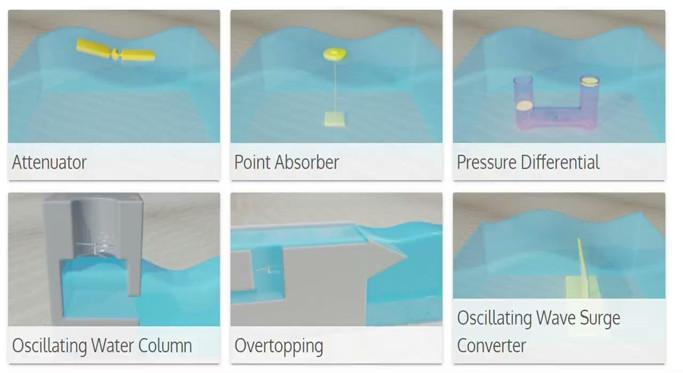
\includegraphics[width=0.9\linewidth]{figs/img0000.png}
	
	{\footnotesize PRIMRE - National Renewable Energy Laboratory}
	
\end{frame}

\begin{frame}
	\frametitle{Motivation: Wave Energy}
	
	\centering
    Relevance to the grid:
	\begin{itemize}
		\item Seasonal profile
		\item Predictability and daily profile
		\item Resource diversity
    \end{itemize}
    Relevance for off-grid projects:
    \begin{itemize}
		\item Offshore co-location
		\item Smaller scale
		\item Other resources not viable
	\end{itemize}
	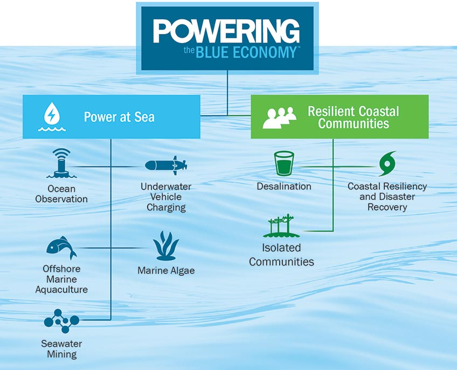
\includegraphics[width=0.9\linewidth]{figs/img0001.png}
	
	{\footnotesize U.S. Department of Energy}
	
\end{frame}


\begin{frame}
	\frametitle{Motivation: Bottlenecks}
	\begin{itemize}
		\item Goal: use early-stage design optimization to inform which      WEC design is    most viable
		      
		\item Low funding
		      
		\item Few ocean deployments
		      
		\item High device costs
		      
		\item Optimization
		      
		\item Value metrics
		      
		\item Alternative markets
		      
		\item High device costs
		      
		\item Value metrics
		      
		\item Optimization
		      
		\item Adapted from Caio et al. 2019
	\end{itemize}
	
\end{frame}



\begin{frame}
	\frametitle{Systems Design}
    We want a simulation and optimization framework that is:
	\begin{itemize}
		\item interdisciplinary
        \item fast
        \item accurate
        \item reproducible
        \item informative
	\end{itemize}
	
\end{frame}